\documentclass{article}
\usepackage{nips13submit_e,times}
\usepackage[utf8x]{inputenc}
\usepackage{amsfonts}
\usepackage{indentfirst}
\usepackage{hyperref}
\usepackage{graphicx}
\usepackage{enumerate}
\usepackage{amsmath}
\usepackage{subfigure} 
\usepackage{amsopn}
\title{Project-II by group TORONTO}
\author{Michalina Pacholska \And Jakub Sygnowski}
\nipsfinalcopy
\begin{document}
\maketitle
\begin{abstract}
This report describes our work on second project done for Machine Learning class at EPFL in Fall 2014. We were given...
\end{abstract}
\section*{Music recommendation system}
\subsection*{Problem and dataset descriptions}
During the project, we were first given a train dataset, which we should analyse and learn our algorithms on, and then, a week before the deadline, we were given a test dataset, for which we should give our predictions. (Following discussions refer to the train dataset). In the dataset, there is information about $A=15082$ artists and $U=1774$ users. Dataset consists of three matrices:
\begin{itemize}
    \item $1\times A$ vector of artists' names - we did not use that.
    \item $U \times A$ matrix of listen count of each artist by every user. This matrix is called $Y_{train}$.
    \item $U \times U$ matrix of social network between users. This matrix is caled $G_{train}$.
\end{itemize}

Both $Y_{train}$ and $G_{train}$ are sparse. Social matrix includes $22904$ ones, which denoted the social connection between users. This mean that our users have on average $12.9109$ friends. $G_{train}$ is symmetric.

In case of listen counts, zero in the matrix meant that the user did not heard of given artist and didn't listen to him, but not necessarily didn't like him. There is $69617$ non-zero entries in the matrix, which constitute $0.26\%$ of it. (Our problem is to predict the listen counts of particular artist for some users).

TODO: test matrices descriptions.

\subsection*{Data analysis and preparation}
We took a look at various distributions of the data and we have found out that:
\begin{enumerate}[1.]
\item Most of the artists have only few distinct listeners. (\ref{fig:artistListeners}). First, we have $1262$ artists for which there don't exist even a single listener, so we cannot predict anything reasonable for them. Then, $90.26\%$ of all the artists have at most $5$ different listeners.
\begin{figure}[!t]
\center
\subfigure[Numbers of artists with various number of listeners. We see that most of the artists have only $1$ or $2$ listeners.]{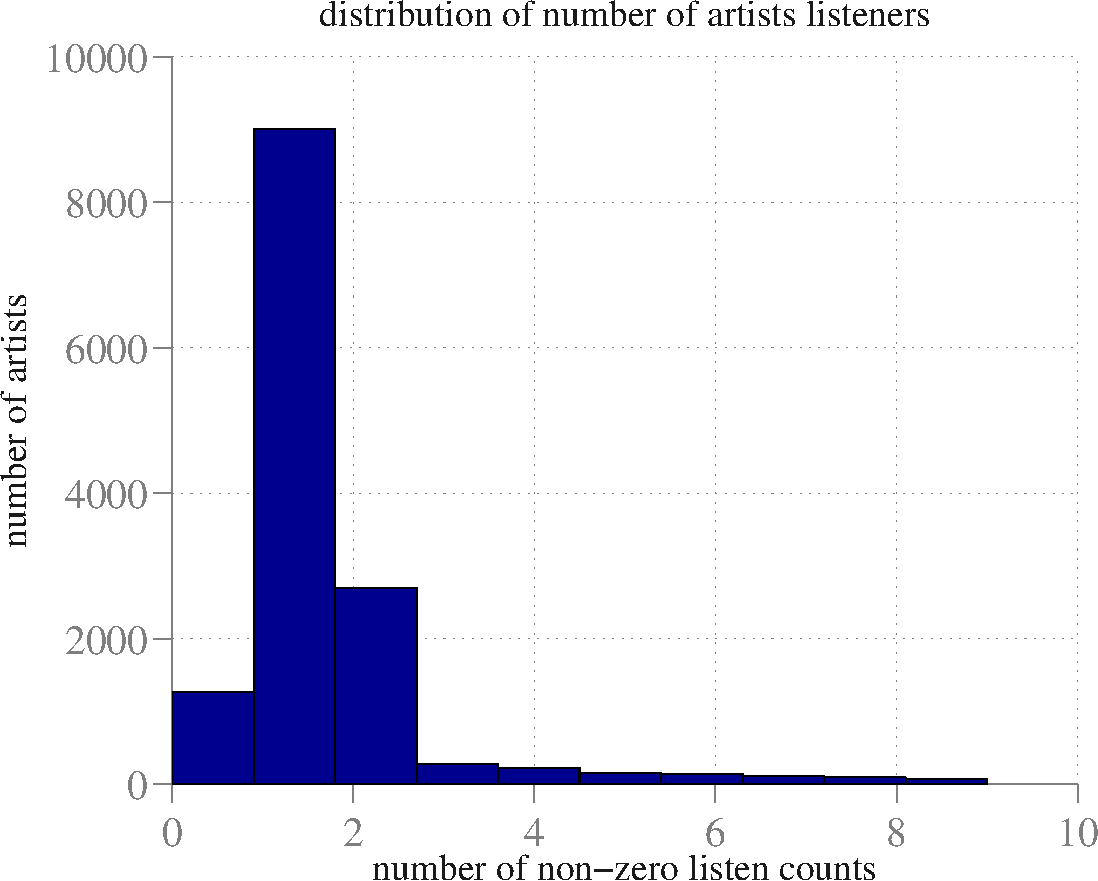
\includegraphics[width=2.5in]{../figures/artist_listeners_count-crop.pdf} \label{fig:artistListeners}}
\hfill
\subfigure[Number of artists for given value of standard deviation of listen counts of users (excluding zero standard deviation)]{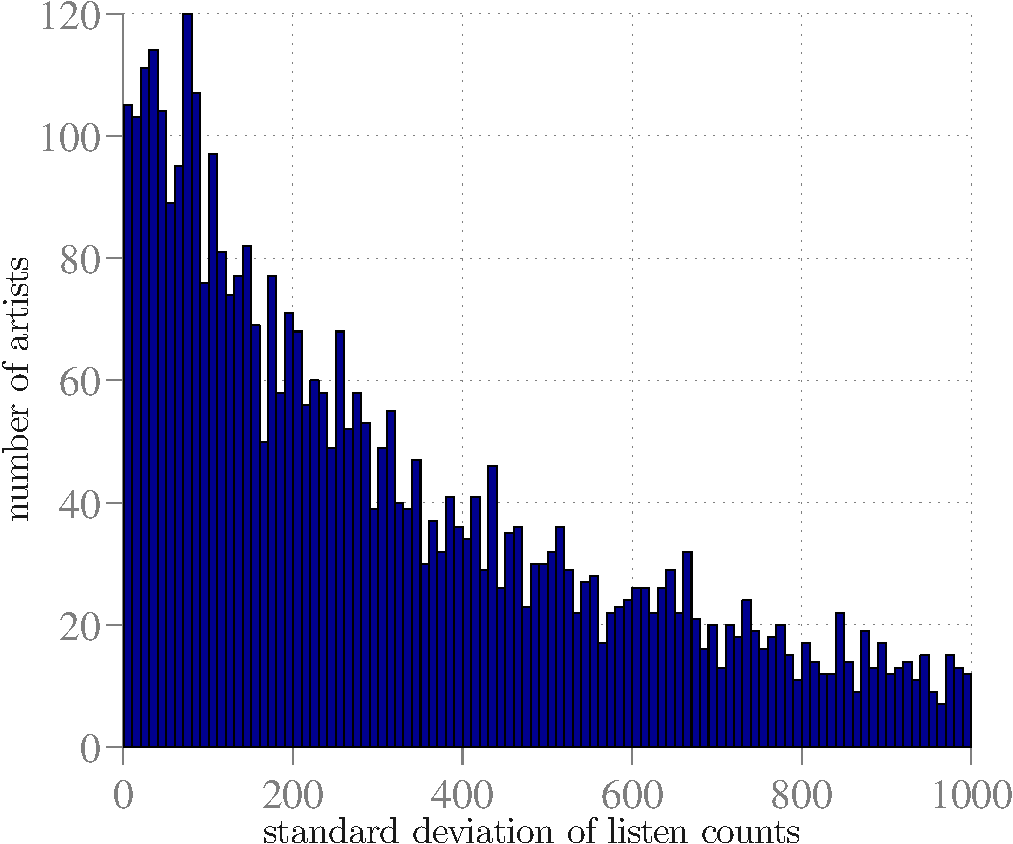
\includegraphics[width=2.5in]{../figures/artist_listeners_std-crop.pdf} \label{fig:artistListenersStd}}
\caption{Analysis of listen counts for given artist}
\end{figure}
\item Among $4812$ artists, who have more than one listener, there is very big standard deviation of listen counts for different users: \ref{fig:artistListenersStd}. E.g. only $93$ of them have standard deviation of listen counts $<10$, and $1017$ have $\mbox{std} < 100$. From this we expect big errors in prediction as in most cases we will have very little data about given artist and the data we will be very uncertain.
\item Distribution of all listen counts (for all artists and all users) is not Gaussian: \ref{fig:listenCounts}. It rather resembles $\frac{1}{x}$ or $e^{-x}$. We tried applying various transformations to normalize the data. We decided to use logarithm, which gave us effect shown on \ref{fig:logListenCounts}. Later, we normalized the data.
%TODO: pisac o tym, ze artysci mieli dziure w sumie odsluchan? brac to pod uwage?
\end{enumerate}
\begin{figure}[!t]
\center
\subfigure[For each (user, artist) listen count value - how many times does it occur in $Y_{train}$ ]{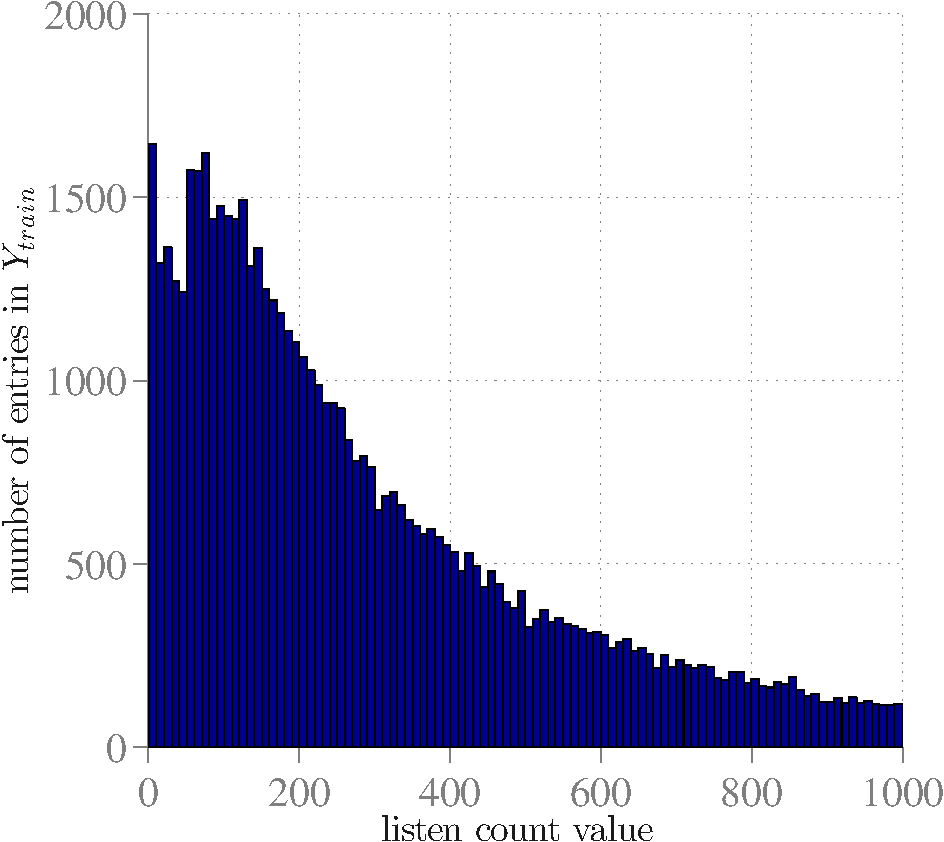
\includegraphics[width=2.5in]{../figures/listen_counts-crop.pdf} \label{fig:listenCounts}}
\hfill
\subfigure[Same histogram as in \ref{fig:listenCounts}, but after taking logarithm of each value]{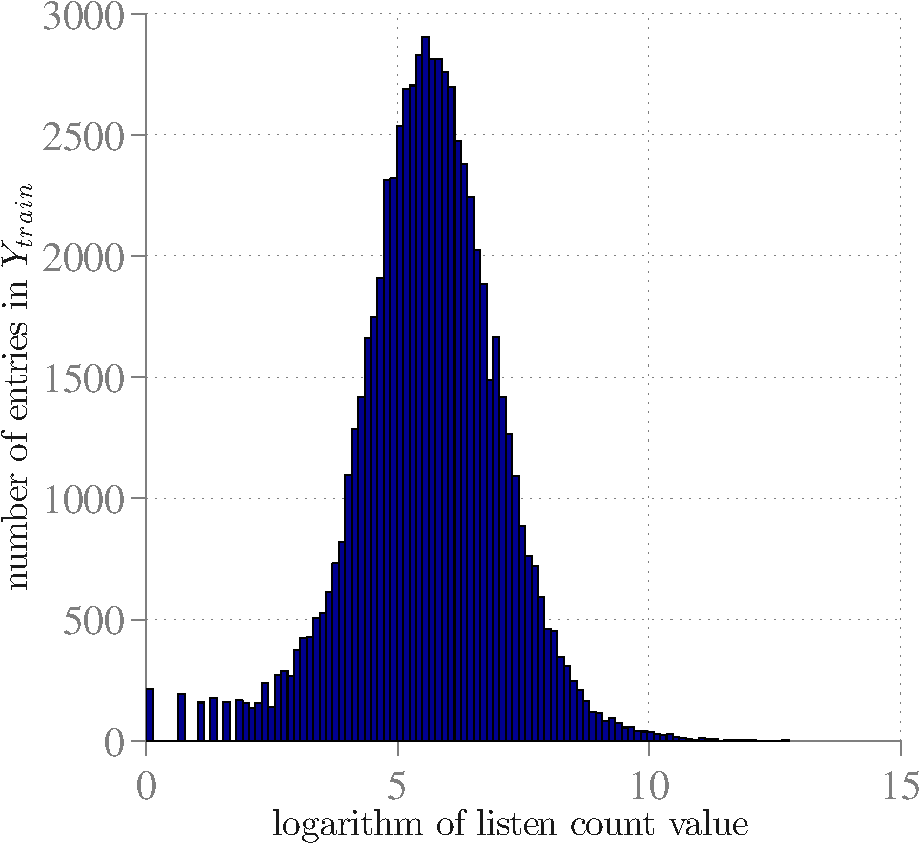
\includegraphics[width=2.5in]{../figures/log_listen_counts-crop.pdf} \label{fig:logListenCounts}}

\caption{Analysis of whole set of listen counts}
\end{figure}
\subsection*{Artist-mean prediction}
First, very simple model we trained, was to predict for each (user, artist) the average listen count of the artist. %TODO: explain cross-validation
 We run it using $k$-fold cross-validation, for $k\in\{2,\ldots, 10\}$, each for $10$ different seeds. We achieved RSME error around $4000$, as shown in the figure: \ref{fig:mean}. This value let us later measure performance of other models. 
 
 We also made a plot to find out for which artists we get the biggest errors: \ref{fig:artistSumError}. It turned out, that errors achieved for artists with at least $10^5$ summaric listen counts (there is only $83 = 0.55\%$ of them), are an order of magnitude bigger than for less commonly listened artists. It is not surprising, as they have bigger variance, but this made as think to put more effort into predicting those "big values". 
\begin{figure}[!t]
\center
\subfigure[Error distribution for different folds.]{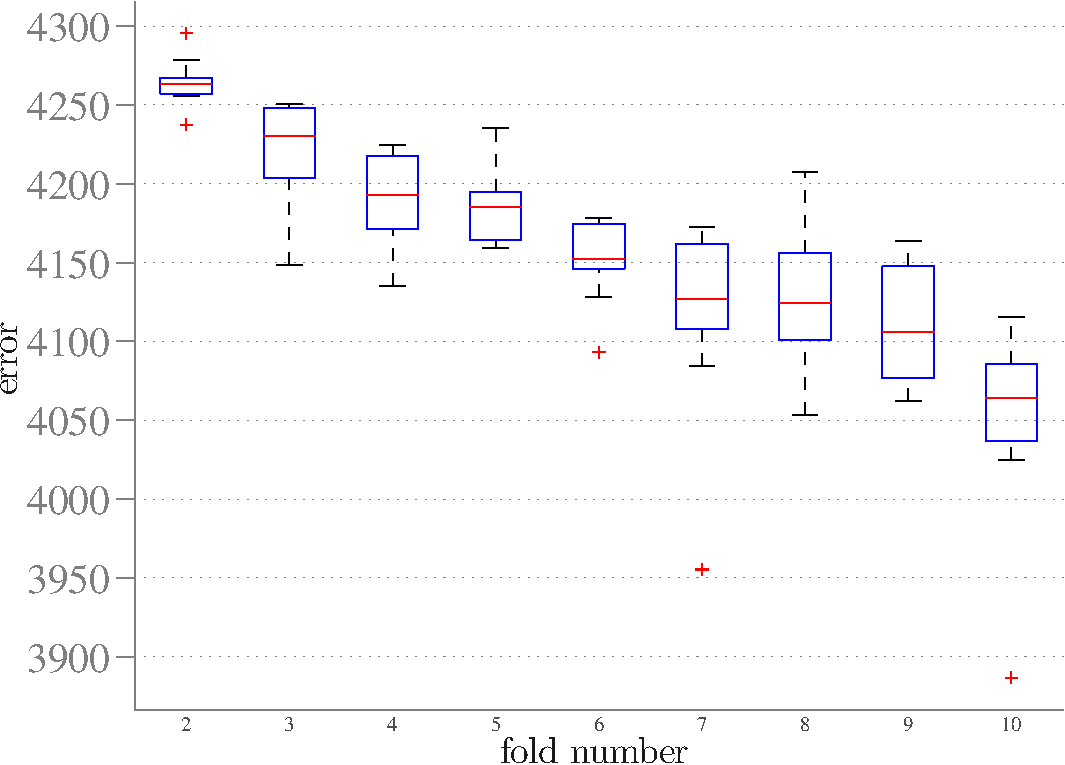
\includegraphics[width=2.5in]{../figures/mean-k-fold-crop.pdf} \label{fig:mean}}
\hfill
\subfigure[Errors all (users, artist) pairs. Point $(x,y)$ in the plot denotes that for some user we got error $y$ and the sum of corresponding artist's listen counts is $y$.]{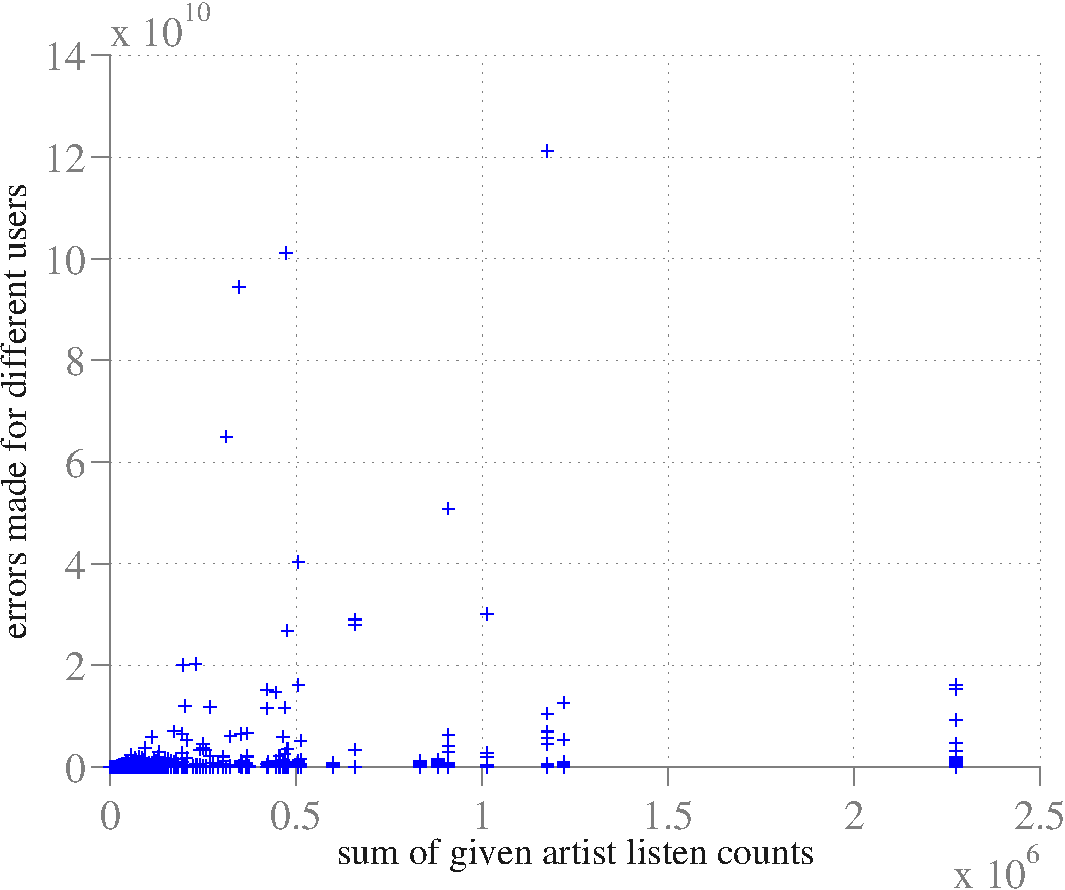
\includegraphics[width=2.5in]{../figures/artist-error-crop.pdf} \label{fig:artistSumError}}
\caption{Results of artist mean prediction}
\end{figure}

Based on this result, as well as the distribution of sums of artist count shown on figure \ref{fig:artistsDist}, we decided to split the dataset into three parts, containing artists which summaric listen counts fit into the intervals:  $[0, 49], [50, 10^5-1], [10^5, \infty)$.
\begin{figure}[!t]
\center
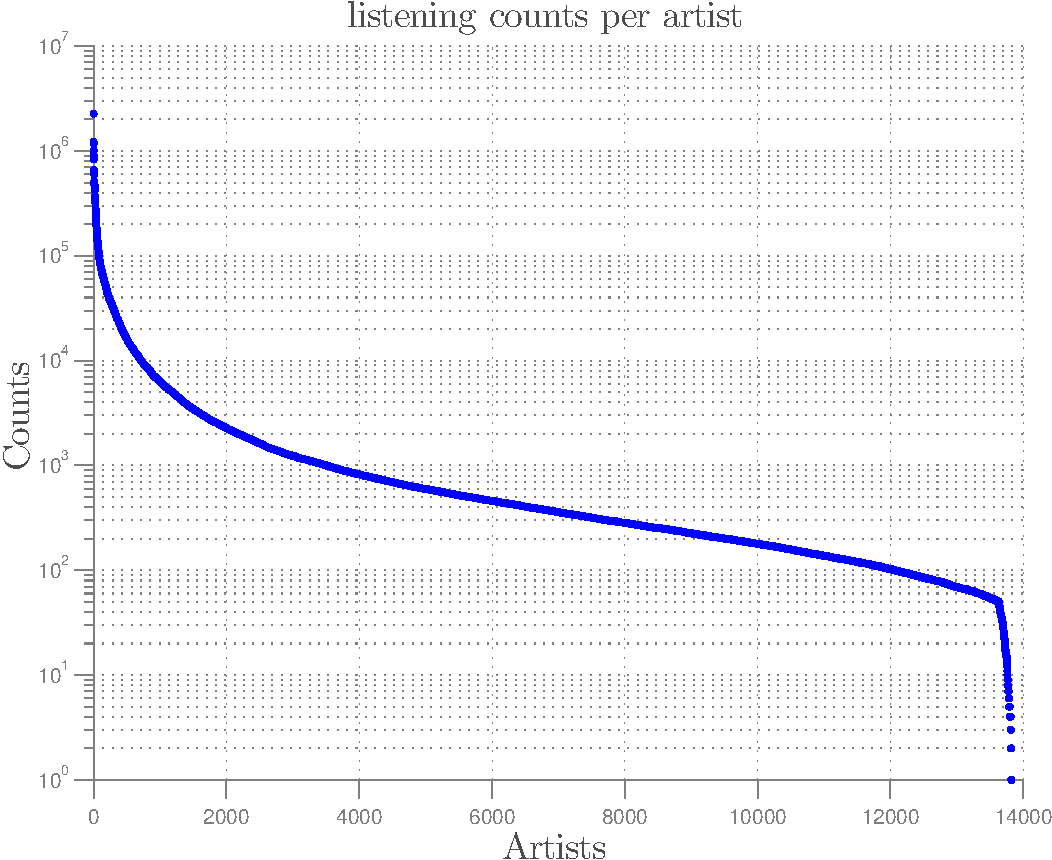
\includegraphics[width=3in]{../figures/artists-distribution-crop.pdf} \label{fig:artistDist}
\caption{Sum of artist count distribution}
\end{figure}
\end{document}
